231. \begin{figure}[ht!]
\center{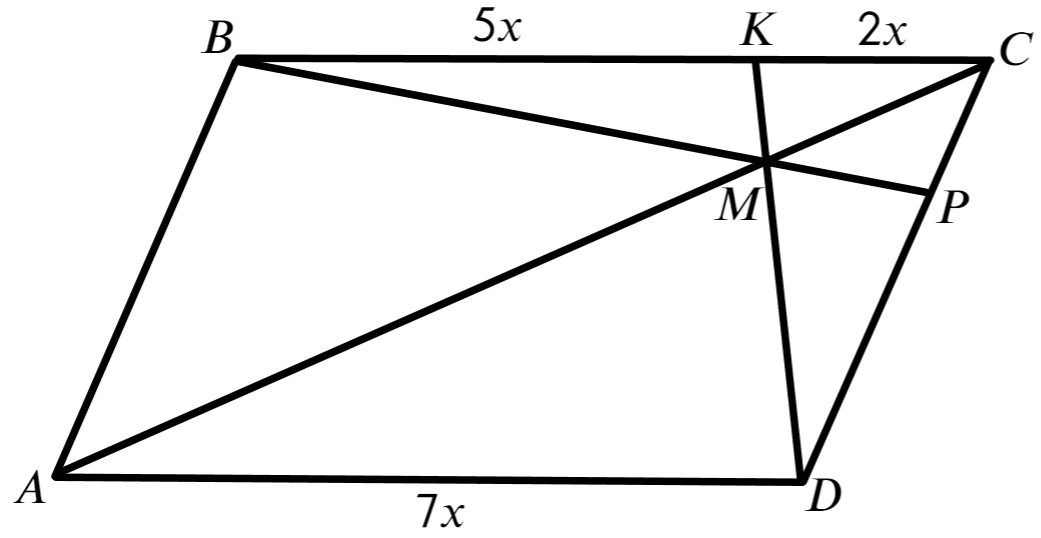
\includegraphics[scale=0.35]{g8-231.png}}
\end{figure}\\
Пусть $BK=5x,$ а $CK=2x,$ тогда $AD=BC=5x+2x=7x.$ Треугольники $CKM$ и $ADM$ подобны по двум углам ($\angle KCM=\angle MAD$ и $\angle CKM=\angle ADM$ как накрест лежащие), поэтому $\cfrac{AM}{CM}=\cfrac{AD}{CK}=\cfrac{7x}{2x}=\cfrac{7}{2}.$ Треугольники $ABM$ и $CPM$ аналогично подобны по двум углам, значит $\cfrac{AB}{CP}=\cfrac{AM}{CM}=\cfrac{7}{2}.$ Тогда $\cfrac{CD}{CP}=\cfrac{AB}{CP}=\cfrac{7}{2},$ значит $CP=\cfrac{2}{7}CD,\ PD=CD-CP=\cfrac{5}{7}CD,\ CP:PD=\cfrac{2}{7}:\cfrac{5}{7}=2:5.$\\
